\subsection{Finding Resonance} \label{B1}

To begin, the NMR spectrometer settings were adjusted explore how they impact an FID signal for the doped water sample. Adjusting the repetition time had no measurable impact on the signal, indicating that water spin-lattice relaxation (regrowth) time is less than (or equal to) the lowest repetition time setting of 0.3 seconds. The receiver gain was not adjusted as increasing it reduced the signal-to-noise ratio of the spectrometer. The receiver phase and the 90 degree pulse dial were adjusted to maximize the signal. Adjusting the 90 degree pulse dial adjusts the amount of time that the sample experiences the applied magnetic field, $B_1$. In our system, the magnetization vector, $\vec{M}$, begins pointing in the direction of $B_0$, which is defined as the $z$-direction. The $B_1$ field is applied in such a way that it rotates the $\vec{M}$ vector into the desired orientation. A 90 degree pulse, as shown in Figure \ref{fig:B1:pulses}, occurs when the $B_1$ field has been applied until $\vec{M}$ points along the $xy$-axis. As our detection system is designed to measure the magnetization along the $x$-axis, the signal is maximized for this type of pulse. \\

Similarly, for a 180 degree pulse $M$ is pointing in the negative $z$-direction and the signal is reduced to approximately zero. For a 270 degree pulse, the signal is minimized (negative peak) as it is pointing along the negative $x$ direction.\\

%The signal decay is caused by the individual spins are spinning at a different frequencies. The different frequencies are caused by inhomogeneities in $B_0$ and the intermolecular forces. If you imagine the spin vectors in a reference frame that is rotating at the Larmour frequency, when $B_1$ field is applied then, for a 90 degree pulse for example, the individual spins all align along the x axis. After the $B_1$ is no longer applied, the vectors start dephasing in the xy plane. The vectors will go out of phase if the spin has a frequency different than the Larmour frequency. Over time, the phasors will completely dephase and add to 0. 

\begin{figure}[H]
    \centering
    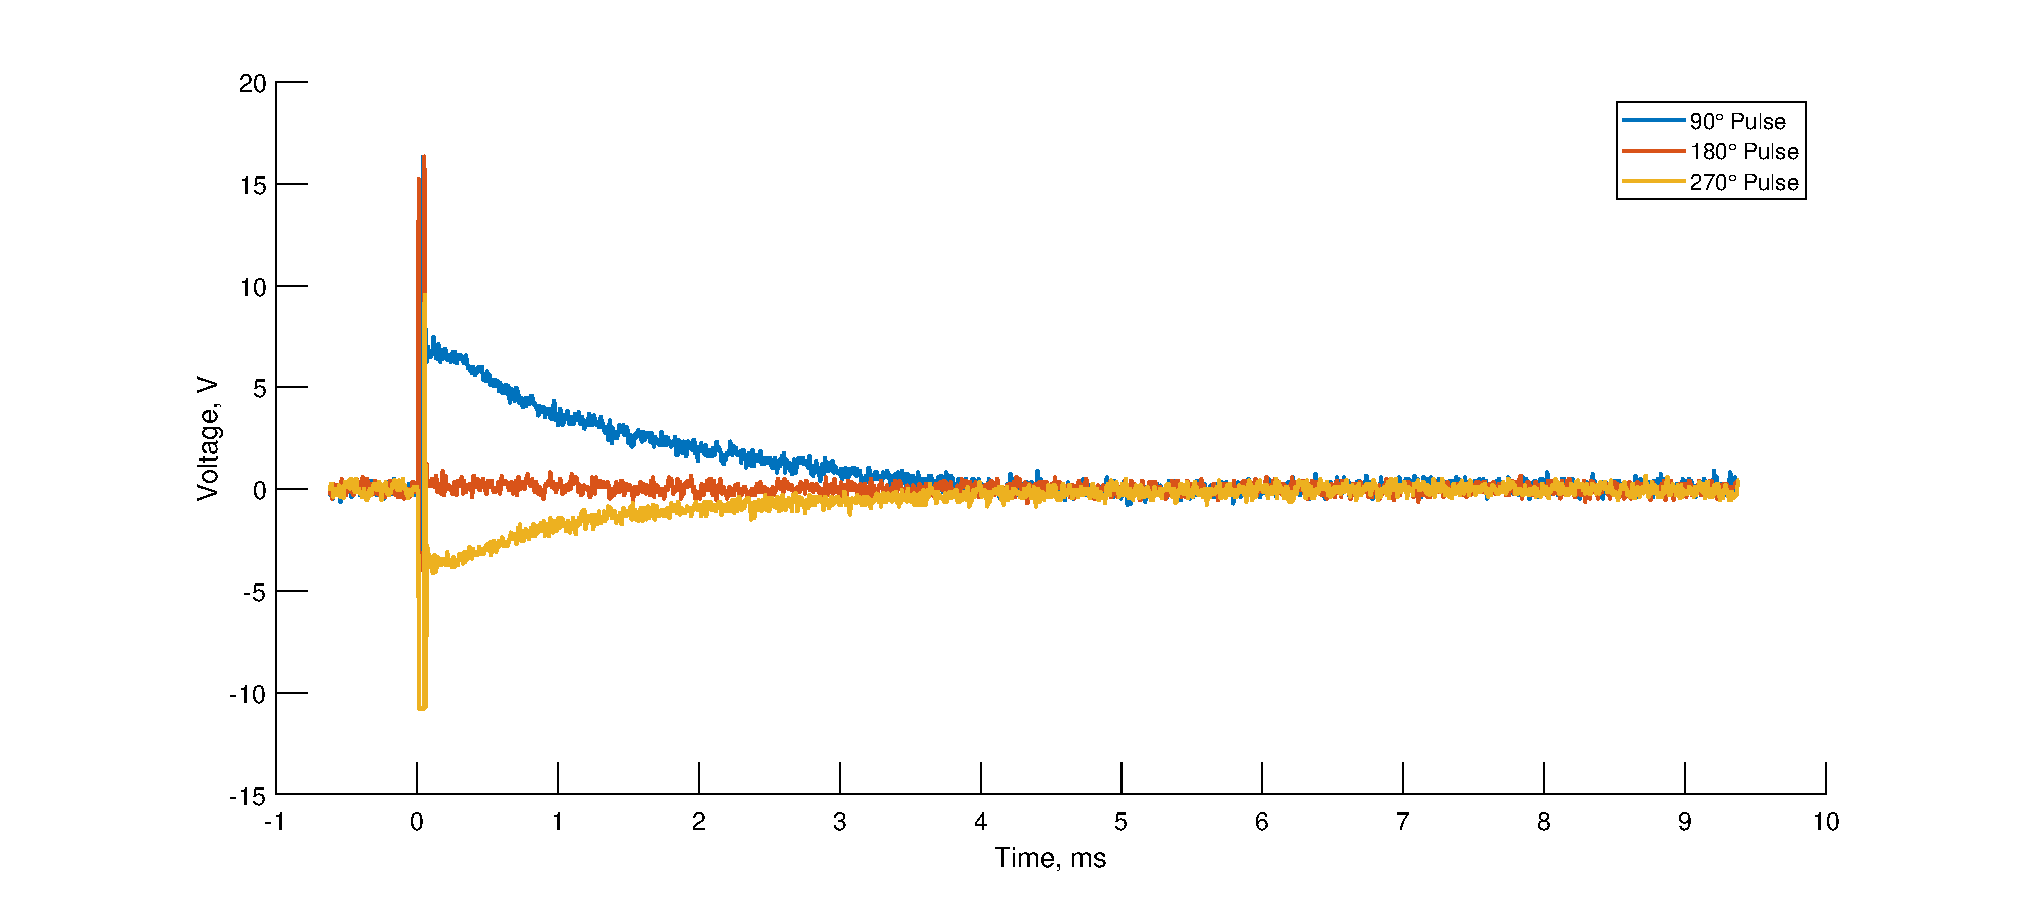
\includegraphics[width=\textwidth]{figures/B1/B1_1.eps}
    \caption{FID of doped water for a 90, 180 and 270 degree pulses.}
    \label{fig:B1:pulses}
\end{figure}


%Figure 5.2 was theoretically supposed to show a 180 degree pulse but the depicted pulse is greater than 180 because there is a negative amplitude, suggesting that there is a negative x component to the signal.